\documentclass[11pt]{article}

\usepackage[letterpaper, margin=1in]{geometry}

\usepackage[spanish]{babel}
\usepackage[utf8]{inputenc}
\usepackage{multirow}
\usepackage{tabularx}
\usepackage{longtable}



%Figuras
\usepackage{graphicx, subfigure}
\usepackage[]{tikz}
\usepackage{pbox}

%Matemática
\usepackage{amsmath}
\usepackage{amssymb}

%Símbolos mate extra (alfabetos, etc.)
\usepackage{mathrsfs}


%Algoritmos
\usepackage{float}
\usepackage{algorithm}
\usepackage{algorithmicx}
\usepackage{algpseudocode}
\usepackage{listings}


\usepackage{color}
\usepackage{hyperref}

\usepackage{mdframed}
\usepackage{tcolorbox}
\usepackage{multicol}
\usepackage{booktabs}
\usepackage{tabulary}
\definecolor{darkblue}{rgb}{0 , 0.054 , 0.196}



\title{Reporte de laboratorio 3}
\author{Laura Rincón Riveros - B55863\\Esteban Vargas Vargas - B16998\\ Grupo 3}

\begin{document}

\maketitle
\hrule
\hrule
\tableofcontents
\hspace{5mm}
\hrule
\hrule

%%%%%%%%%%%%%%%%%%%%%%%%%%%%%%%%%%%%
\section{Introducción}
%%%%%%%%%%%%%%%%%%%%%%%%%%%%%%%%%%%%

En el presente laboratorio se utilizó una clase plantilla y la sobrecarga de operadores. Como se presenta a continuación:


\newpage
%%%%%%%%%%%%%%%%%%%%%%%%%%%%%%%%%%%%
\section{Desarrollo}
%%%%%%%%%%%%%%%%%%%%%%%%%%%%%%%%%%%%

%%%%%%%%%%%%%%%%%%%%%%
\subsection{Clase Calculadora}
%%%%%%%%%%%%%%%%%%%%%%

Se creó una clase emplantillada llamada Calculadora, en la cuál se definieron las funciones básicas suma, resta, multiplicación, división e impresión. Esta clase se creó emplantillada para que pudiera realizar operaciones sobre distintos tipos de datos, no sólo tipos primitivos como enteros y decimales sino que también objetos creados como una fracción, una matriz o un polinomio. Esta se presenta a continuación: 

\begin{figure}[H]
\centering
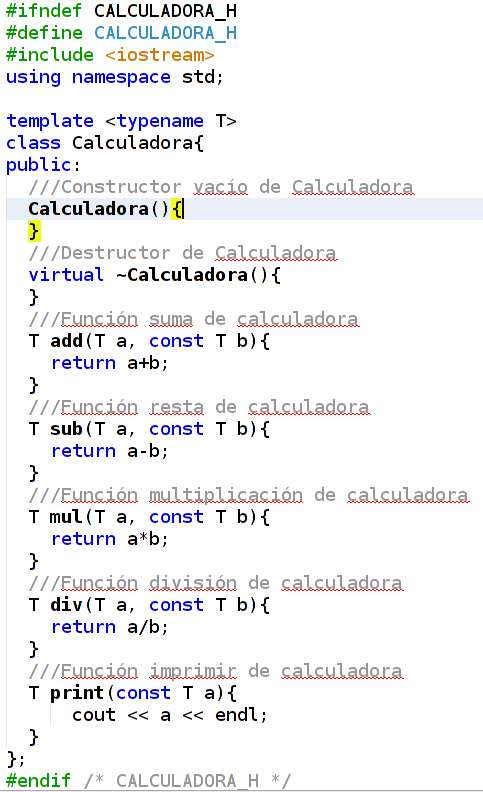
\includegraphics[height=15cm, width=\textwidth]{img/HeaderCalculadora.png}
\caption{Calculadora.h}
\label{fig:calch}
\end{figure}

%\begin{figure}[H]
%\centering
%\subfigure[Figura.h]{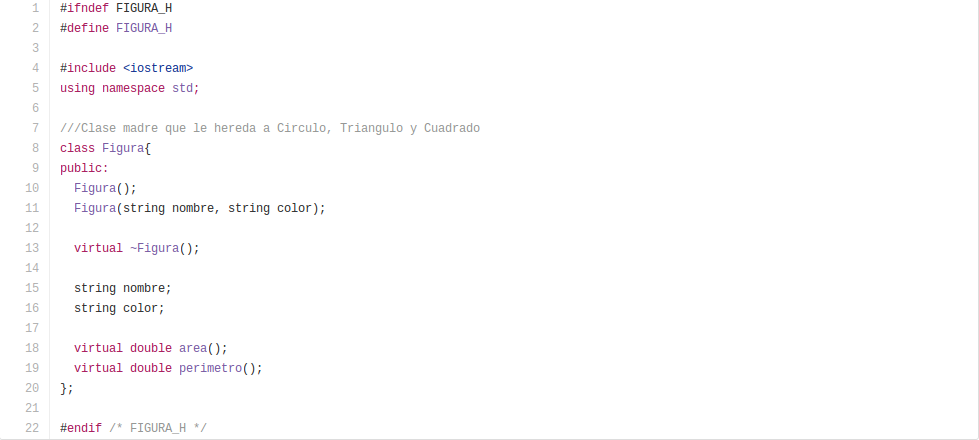
\includegraphics[height=8cm, width=\textwidth]{img/figurah.png}}
%\subfigure[Figura.cpp]{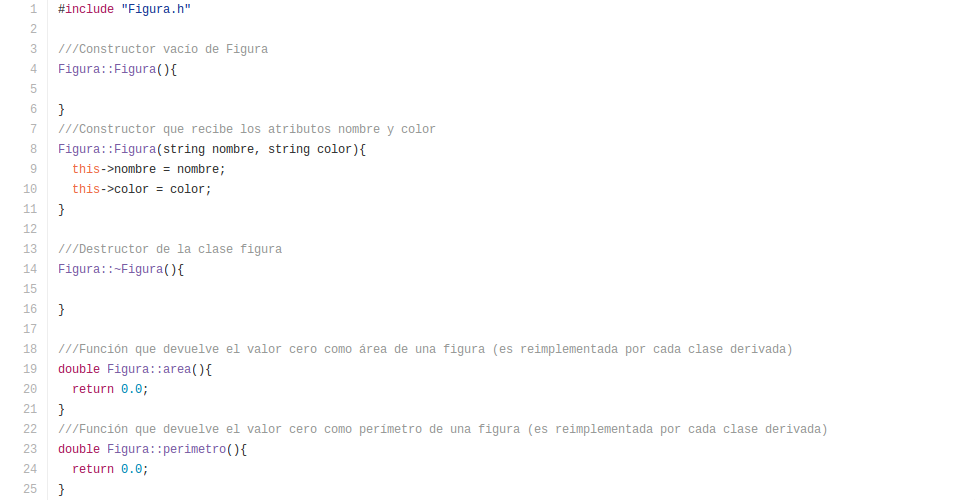
\includegraphics[height=5.5cm, width=\textwidth]{img/figuracpp.png}}
%\caption{Clase base Figura}
%\label{fig:plantilla}
%\end{figure}

\newpage
%%%%%%%%%%%%%%%%%%%%%%
\subsection{Clase Fracción}
%%%%%%%%%%%%%%%%%%%%%%

La clase Fracción cuenta con los atributos: 
\begin{itemize}
\item Numerador (int)
\item Denominador (int)
\end{itemize}

A continuación se muestra la declaración de los atributos y funciones de la clase Fracción, del archivo encabezado de Fracción.

\begin{figure}[H]
\centering
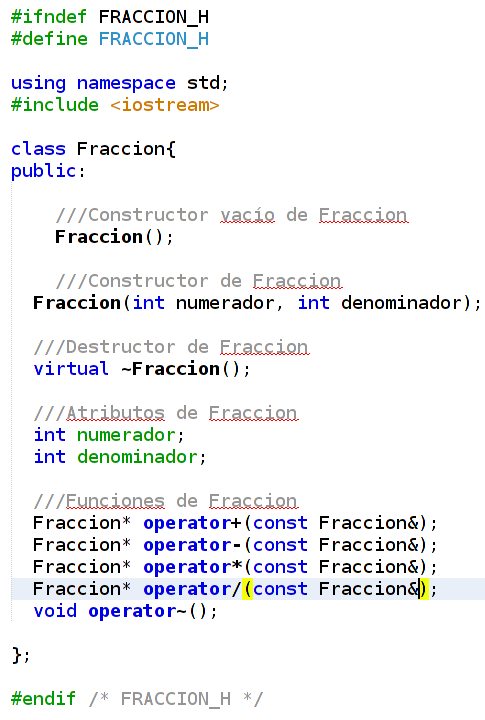
\includegraphics[height=15cm, width=\textwidth]{img/HeaderFraccion.png}
\caption{Fracción.h}
\label{fig:frach}
\end{figure}

La implementación de la sobrecarga de operadores para este tipo de objeto se realizó de la siguiente manera:
\begin{itemize}
\item Suma: Se tomaron en cuenta 3 casos (Teniendo F1 y F2):
\begin{enumerate}
\item Si los denominadores de F1 y F2 son iguales el resultado es una fracción con el denominador y el numerador igual a la suma del numerador de F1 y F2.
\item Si los denominadores de F1 y F2 son distintos, el de F1 es mayor que el de F2 y el de F1 es divisible entre el de F2 entonces el resultado es una fracción con el denominador igual al denominador de F1 y el numerador es igual a la suma del numerador de F1 mas el numerador de F1 multiplicado por la división del denominador de F1 y F2.
\item Si los denominadores D1 y D2 de F1 y F2 son distintos pero no son divisibles entre ellos, entonces el resultado es una fracción con un denominador DS igual a la multiplicación de D1 y D2. El numerador del resultado se obtiene sumando la multiplicación de la división de DS entre D1 y D2 multiplicado por su respectivo numerador. 
\end{enumerate}
\item Resta: Se implementó de igual manera que la suma pero realizando una resta.
\item Multiplicación: Se obtuvo multiplicando los numeradores y denominadores de las dos fracciones a multiplicar.
\item División: Sea una fraccion F1 con denominador D1 y numerador N1, y sea una fraccion F2 con denominador D2 y numerador N2, el resultado se compone de un numerador N=N1*D2 y un numerador D=D1*N2. 
\item Impresión: Se imprime el numerador y el denominador, separados por un "/".
\end{itemize}

\newpage 
%%%%%%%%%%%%%%%%%%%%%%
\subsection{Clase Matriz}
%%%%%%%%%%%%%%%%%%%%%%
La clase Matriz cuenta con los atributos:
\begin{itemize}
\item Número de filas (int)
\item Número de columnas (int)
\item Contenido (int**)
\end{itemize}
A continuación se muestra la declaración de los atributos y funciones de la clase Matriz, del archivo encabezado de Matriz.


\begin{figure}[H]
\centering
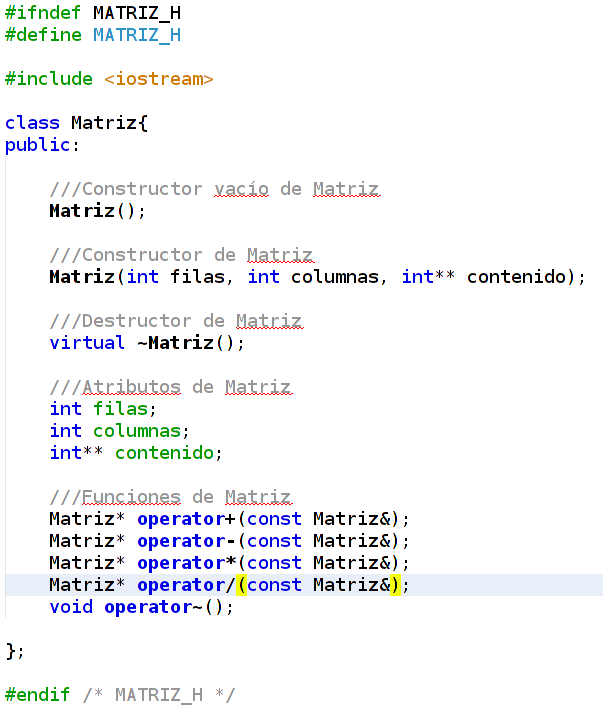
\includegraphics[height=15cm, width=\textwidth]{img/HeaderMatriz.png}
\caption{Matriz.h}
\label{fig:math}
\end{figure}


La implementación de la sobrecarga de operadores para este tipo de objeto se realizó de la siguiente manera:
\begin{itemize}
\item Suma: Luego de comprobar que las dimensiones de las dos matrices sean las mismas, se suma entrada por entrada.
\item Resta: Luego de comprobar que las dimensiones de las dos matrices sean las mismas, se resta entrada por entrada.
\item Multiplicación: Luego de comprobar que el número de columnas de la primera matriz sea igual al número de filas de la segunda matriz, se crea una matriz nueva del número de filas de la primera matriz y del número de columnas de la segunda. Posteriormente se procede a llenar esta nueva matriz resultado con el algoritmo conocido de multiplicación de matrices.
\item División: Luego de comprobar que las dimensiones de las dos matrices sean las mismas, se divide entrada por entrada.
\item Impresión: Mediante el uso de 2 \textit{for} se recorre toda la matriz entrada por entrada y se despliega en consola. 
\end{itemize}
%%%%%%%%%%%%%%%%%%%%%%
\newpage 
\subsection{Clase Polinomio}
La clase polinomio cuenta con los atributos:
\begin{itemize}
\item Grado Mayor (int)
\item Coeficientes (int*)
\end{itemize}

A continuación se muestra la declaración de los atributos y funciones de la clase Polinomio, del archivo encabezado de Polinomio.

\begin{figure}[H]
\centering
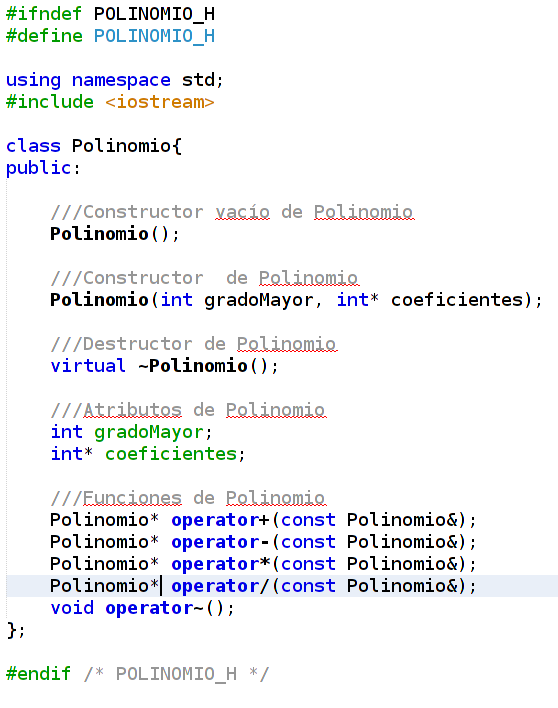
\includegraphics[height=15cm, width=\textwidth]{img/HeaderPolinomio.png}
\caption{Polinomio.h}
\label{fig:polh}
\end{figure}


La implementación de la sobrecarga de operadores para este tipo de objeto se realizó de la siguiente manera:
\begin{itemize}
\item Suma: Se consideraron dos casos para verificar cuál de los dos polinomios tenía mayor grado. A partir de ahí, se creó un objeto nuevo con el tamaño del puntero de  coeficiente adecuado; se sumaban los coeficientes de ambos polinomios desde el grado 0 hasta el grado del polinomio menor y luego se agregaban los coeficientes faltantes del polinomio mayor.
\item Resta: Se siguió el procedimiento de suma pero restando los coeficientes de los polinomios, esta vez.
\item Multiplicación: Para la multiplicación se consideró que el polinomio resultante sería de un grado equivalente a la suma de los grados de los polinomios que la función recibe. Con lo anterior, se procedió a llenar el nuevo polinomio resultante, con la multiplicación de cada término y la suma de los téminos del mismo grado.
\item División: Para la división se emplentó un algoritmo de los siguientes pasos:

Se divide el primer término del dividendo (this$->$coeficientes) entre el primer término del divisor(other.coeficientes), para obtener el primer término del cociente (Result.coeficientes). Se Multiplica el divisor por el primer término del cociente y se resta al dividendo el resultado anterior para conseguir el primer residuo parcial (Temp.coeficientes). 
Y se repite el procedimiento haciendo ahora dividendo el primer resto parcial.La división finaliza cuando el grado del resto es menor que el grado del divisor. 
\item Impresión: Para el caso de la impresión,se recorrió el arreglo de coeficientes, se imprimía el valor y la posición del arreglo como el grado del polinomio adicionando un $+$ entre cada término.
\end{itemize}
%%%%%%%%%%%%%%%%%%
%%%%%%%%%%%%%%%%%%%%%%
\subsection{Main}
%%%%%%%%%%%%%%%%%%%%%%
En el archivo main se crearon pares de los objetos mencionados Matriz, Polinomio y Fracción para aplicarle las funciones de suma, resta, multiplicación y división; posibles gracias a la sobrecarga de operadores. Para aplicarle las funciones a los objetos se hizo uso de la clase emplantillada calculadora, la cual permite introducirle cualquier tipo de dato. A continuación se ilustra lo anterior.

\newpage
%%%%%%%%%%%%%%%%%%%%%%
\subsection{Diagrama de clases}
%%%%%%%%%%%%%%%%%%%%%%
Para una mejor visualización de la composición de las clases se presentan a continuación los diagramas respectivos.

\begin{figure}[htbp]
\centering
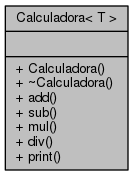
\includegraphics[width=0.35\textwidth]{img/UMLcalc.png}
\caption{\label{fig:umlcalc} UML Calculadora}
\end{figure}

\begin{figure}[htbp]
\centering
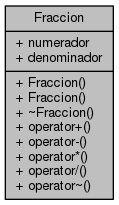
\includegraphics[width=0.25\textwidth]{img/UMLFrac.png}
\caption{\label{fig:umlfrac} UML Fracción}
\end{figure}

\begin{figure}[htbp]
\centering
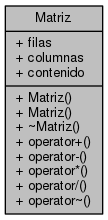
\includegraphics[width=0.25\textwidth]{img/UMLmat.png}
\caption{\label{fig:umlmat} UML Matriz}
\end{figure}

\begin{figure}[htbp]
\centering
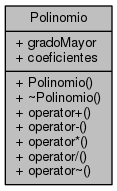
\includegraphics[width=0.25\textwidth]{img/UMLpol.png}
\caption{\label{fig:umlpol} UML Polinomio}
\end{figure}
 
\newpage
%%%%%%%%%%%%%%%%%%%%%%%%%%%%%%%%
\section{Conclusiones}
%%%%%%%%%%%%%%%%%%%%%%%%%%%%%%%%
\begin{itemize}
\item Se empleó la programación orientada a objetos para el uso de clases.
\item Se construyó una clase emplantillada capaz de manipular distintos tipos de datos (primitivos y objetos).
\item Se sobrecargaron distintos operadores para poder efectuar operaciones básicas a matrices, polinomios y fracciones. 
\end{itemize}
\end{document}
